\section{Exercices d'application}

\rubrique{Conversion degrés-radians et cercle trigonométrique}

\exo{}\diff{1}
Convertir en radians les mesures suivantes : $30^\circ$, $45^\circ$, $60^\circ$, $90^\circ$, $120^\circ$, $180^\circ$, $270^\circ$, $360^\circ$.

\exo{}\diff{1}
Convertir en degrés les mesures suivantes : $\dfrac{\pi}{6}$, $\dfrac{\pi}{4}$, $\dfrac{\pi}{3}$, $\dfrac{2\pi}{3}$, $\dfrac{3\pi}{4}$, $\dfrac{5\pi}{6}$, $\pi$, $\dfrac{3\pi}{2}$.

\exo{}\diff{1}
Placer sur le cercle trigonométrique les points correspondant aux réels suivants :
\[
\frac{\pi}{6},\quad \frac{5\pi}{6},\quad -\frac{2\pi}{3},\quad \frac{7\pi}{4},\quad -\frac{\pi}{4},\quad \frac{11\pi}{6}.
\]

\rubrique{Mesure principale d'un angle orienté}

\exo{}\diff{2}
Déterminer la mesure principale des angles orientés dont une mesure est donnée :
\[
\frac{15\pi}{4},\quad -\frac{23\pi}{6},\quad \frac{37\pi}{3},\quad -\frac{19\pi}{2}.
\]

\exo{}\diff{2}
Soit $\alpha$ un angle orienté tel que $\alpha \equiv \dfrac{5\pi}{6} \pmod{2\pi}$. Donner trois autres mesures de $\alpha$, dont une négative.

\rubrique{Lignes trigonométriques et valeurs remarquables}

\exo{}\diff{1}
Calculer les valeurs exactes de :
\[
\cos\frac{\pi}{6},\quad \sin\frac{\pi}{4},\quad \tan\frac{\pi}{3},\quad \cos\frac{3\pi}{4},\quad \sin\frac{5\pi}{6},\quad \tan\frac{2\pi}{3}.
\]

\exo{}\diff{2}
Sachant que $\sin x = \dfrac{3}{5}$ et que $x \in \left]\dfrac{\pi}{2};\pi\right[$, calculer $\cos x$ et $\tan x$.

\exo{}\diff{2}
Sachant que $\cos x = -\dfrac{2}{3}$ et que $x \in \left]\pi;\dfrac{3\pi}{2}\right[$, calculer $\sin x$ et $\tan x$.

\rubrique{Relations fondamentales et angles associés}

\exo{}\diff{2}
Simplifier les expressions suivantes :
\[
A = \cos\left(\frac{\pi}{2}+x\right) + \sin(\pi-x) - \cos(\pi+x) + \sin\left(\frac{3\pi}{2}-x\right).
\]

\exo{}\diff{2}
Simplifier :
\[
B = \frac{\sin\left(\frac{\pi}{2}+x\right)\cos(\pi-x)}{\cos\left(\frac{3\pi}{2}+x\right)\sin(\pi+x)}.
\]

\exo{}\diff{3}
On donne $\cos a = \dfrac{1}{3}$ avec $a \in \left]0;\dfrac{\pi}{2}\right[$. Calculer $\cos\left(\dfrac{\pi}{3}+a\right)$ et $\sin\left(\dfrac{\pi}{6}-a\right)$.

\rubrique{Équations trigonométriques simples}

\exo{}\diff{2}
Résoudre dans $\R$ les équations suivantes :
\[
\cos x = \frac{\sqrt{2}}{2},\qquad \sin x = -\frac{1}{2},\qquad \tan x = \sqrt{3}.
\]

\exo{}\diff{3}
Résoudre dans $]-\pi;\pi]$ l'équation : $\cos\left(2x+\dfrac{\pi}{3}\right) = \dfrac{1}{2}$.

\section{Exercices d'entraînement}

\rubrique{Conversion et repérage}

\exo{}\diff{1}
Convertir en radians : $15^\circ$, $72^\circ$, $150^\circ$, $225^\circ$, $300^\circ$.

\exo{}\diff{1}
Convertir en degrés : $\dfrac{\pi}{5}$, $\dfrac{2\pi}{5}$, $\dfrac{7\pi}{12}$, $\dfrac{11\pi}{18}$, $\dfrac{13\pi}{9}$.

\exo{}\diff{1}
Placer sur le cercle trigonométrique les points correspondant aux réels : $\dfrac{\pi}{3}$, $\dfrac{2\pi}{3}$, $\dfrac{4\pi}{3}$, $\dfrac{5\pi}{3}$, $-\dfrac{\pi}{6}$, $-\dfrac{5\pi}{6}$.

\exo{}\diff{2}
Déterminer la mesure principale des angles : $\dfrac{25\pi}{3}$, $-\dfrac{31\pi}{4}$, $\dfrac{47\pi}{6}$, $-\dfrac{53\pi}{2}$.

\exo{}\diff{2}
Soit $\alpha$ un angle orienté tel que $\alpha \equiv -\dfrac{3\pi}{4} \pmod{2\pi}$. Donner trois autres mesures de $\alpha$, dont une positive.

\rubrique{Calculs de lignes trigonométriques}

\exo{}\diff{1}
Calculer les valeurs exactes de : $\cos\dfrac{\pi}{3}$, $\sin\dfrac{\pi}{6}$, $\tan\dfrac{\pi}{4}$, $\cos\dfrac{2\pi}{3}$, $\sin\dfrac{3\pi}{4}$, $\tan\dfrac{5\pi}{6}$.

\exo{}\diff{2}
Sachant que $\sin x = -\dfrac{4}{5}$ et que $x \in \left]\pi;\dfrac{3\pi}{2}\right[$, calculer $\cos x$ et $\tan x$.

\exo{}\diff{2}
Sachant que $\cos x = \dfrac{5}{13}$ et que $x \in \left]-\dfrac{\pi}{2};0\right[$, calculer $\sin x$ et $\tan x$.

\exo{}\diff{2}
Sachant que $\tan x = 2$ et que $x \in \left]0;\dfrac{\pi}{2}\right[$, calculer $\sin x$ et $\cos x$.

\exo{}\diff{3}
On donne $\sin a = \dfrac{2}{3}$ avec $a \in \left]\dfrac{\pi}{2};\pi\right[$. Calculer $\cos a$, $\tan a$, puis $\cos\left(\dfrac{\pi}{4}+a\right)$ et $\sin\left(\dfrac{\pi}{3}+a\right)$.

\rubrique{Simplifications et expressions}

\exo{}\diff{2}
Simplifier :
\[
C = \cos\left(\frac{3\pi}{2}-x\right) + \sin(\pi+x) - \cos\left(\frac{\pi}{2}-x\right) + \sin\left(\frac{3\pi}{2}+x\right).
\]

\exo{}\diff{2}
Simplifier :
\[
D = \frac{\cos\left(\frac{3\pi}{2}+x\right)\sin\left(\frac{\pi}{2}-x\right)}{\sin(\pi-x)\cos\left(\frac{\pi}{2}+x\right)}.
\]

\exo{}\diff{2}
Simplifier :
\[
E = \cos^2 x - \sin^2 x + 2\sin x \cos x \tan x.
\]

\exo{}\diff{3}
Montrer que pour tout réel $x$ :
\[
(\cos x + \sin x)^2 + (\cos x - \sin x)^2 = 2.
\]

\exo{}\diff{3}
Montrer que pour tout réel $x$ :
\[
\frac{1}{\cos^2 x} - \tan^2 x = 1.
\]

\rubrique{Équations trigonométriques}

\exo{}\diff{2}
Résoudre dans $\R$ : $\cos x = -\dfrac{\sqrt{3}}{2}$, $\sin x = \dfrac{\sqrt{2}}{2}$, $\tan x = -1$.

\exo{}\diff{2}
Résoudre dans $]-\pi;\pi]$ : $\sin\left(3x-\dfrac{\pi}{4}\right) = \dfrac{\sqrt{3}}{2}$.

\exo{}\diff{3}
Résoudre dans $[0;2\pi[$ : $\cos^2 x - \sin^2 x = \dfrac{1}{2}$.

\exo{}\diff{3}
Résoudre dans $\R$ : $2\cos^2 x - 3\cos x + 1 = 0$.

\section{Problèmes type Probatoire/Bac}

\sujetbac[Problème 1 : Cercle trigonométrique et angles associés]
\`A l'aide du cercle trigonométrique, répondre aux questions suivantes.
\begin{enumerate}[label=\arabic*)]
\item Placer les points $M_1$, $M_2$, $M_3$, $M_4$ du cercle trigonométrique correspondant respectivement aux réels $\dfrac{\pi}{6}$, $\dfrac{5\pi}{6}$, $\dfrac{7\pi}{6}$, $\dfrac{11\pi}{6}$.
\item Donner les coordonnées de ces points.
\item En déduire les valeurs exactes de $\cos\dfrac{5\pi}{6}$, $\sin\dfrac{5\pi}{6}$, $\cos\dfrac{7\pi}{6}$, $\sin\dfrac{7\pi}{6}$.
\item Simplifier l'expression :
\[
F = \cos\left(\frac{\pi}{6}+x\right) + \cos\left(\frac{5\pi}{6}+x\right) + \cos\left(\frac{7\pi}{6}+x\right) + \cos\left(\frac{11\pi}{6}+x\right).
\]
\end{enumerate}

\sujetbac[Problème 2 : Lignes trigonométriques et applications]
Un avion décolle de l'aéroport international de Douala. Il suit une trajectoire rectiligne faisant un angle de $30^\circ$ avec le sol. Après avoir parcouru $2000$ mètres, il se trouve à une altitude $h$.
\begin{enumerate}[label=\arabic*)]
\item Faire un schéma de la situation.
\item Exprimer $h$ en fonction de la distance parcourue $d$ et de l'angle.
\item Calculer $h$ (on donnera la valeur exacte puis une valeur approchée au mètre près).
\item L'avion poursuit sa montée avec le même angle. Quelle distance doit-il parcourir pour atteindre une altitude de $3000$ mètres ?
\end{enumerate}

\sujetbac[Problème 3 : Résolution d'équations trigonométriques]
On considère l'équation $(E) : 2\sin^2 x - 3\sin x + 1 = 0$.
\begin{enumerate}[label=\arabic*)]
\item Résoudre dans $\R$ l'équation $2X^2 - 3X + 1 = 0$.
\item En déduire les solutions de $(E)$ dans $\R$.
\item Donner les solutions de $(E)$ appartenant à l'intervalle $]-\pi;\pi]$.
\item Représenter ces solutions sur le cercle trigonométrique.
\end{enumerate}

\section{Corrigés}

\corrige{de l'exercice 1}
\[
30^\circ = \frac{\pi}{6},\quad 45^\circ = \frac{\pi}{4},\quad 60^\circ = \frac{\pi}{3},\quad 90^\circ = \frac{\pi}{2},\quad 120^\circ = \frac{2\pi}{3},\quad 180^\circ = \pi,\quad 270^\circ = \frac{3\pi}{2},\quad 360^\circ = 2\pi.
\]

\corrige{de l'exercice 2}
\[
\frac{\pi}{6}=30^\circ,\quad \frac{\pi}{4}=45^\circ,\quad \frac{\pi}{3}=60^\circ,\quad \frac{2\pi}{3}=120^\circ,\quad \frac{3\pi}{4}=135^\circ,\quad \frac{5\pi}{6}=150^\circ,\quad \pi=180^\circ,\quad \frac{3\pi}{2}=270^\circ.
\]

\corrige{de l'exercice 3}
\begin{center}
\begin{illus}
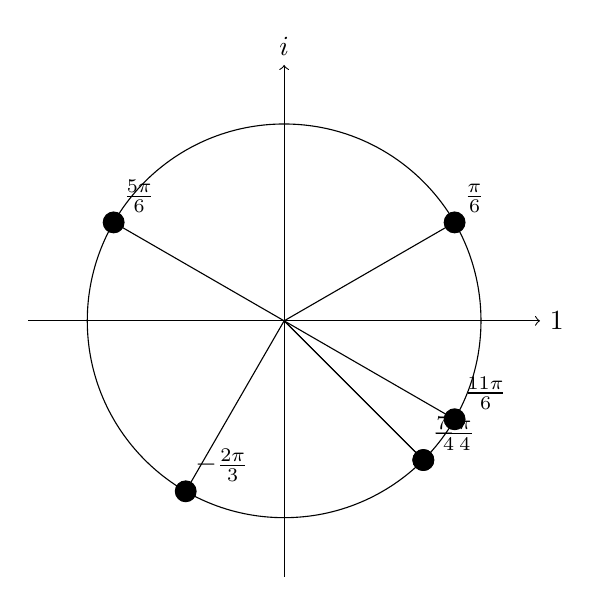
\begin{tikzpicture}[scale=2.5]
\draw[->] (-1.3,0) -- (1.3,0) node[right] {$1$};
\draw[->] (0,-1.3) -- (0,1.3) node[above] {$i$};
\draw (0,0) circle (1);
\foreach \a/\lab in {30/{$\frac{\pi}{6}$},150/{$\frac{5\pi}{6}$},-120/{$-\frac{2\pi}{3}$},315/{$\frac{7\pi}{4}$},-45/{$-\frac{\pi}{4}$},330/{$\frac{11\pi}{6}$}} {
\draw (0,0) -- (\a:1);
\filldraw (\a:1) circle (1.5pt) node[above right] {\lab};
}
\end{tikzpicture}
\fig{Placement des points sur le cercle trigonométrique}
\end{illus}
\end{center}

\corrige{de l'exercice 4}
\begin{itemize}
\item $\dfrac{15\pi}{4} = \dfrac{15\pi}{4} - 2\pi = \dfrac{15\pi}{4} - \dfrac{8\pi}{4} = \dfrac{7\pi}{4}$. Comme $-\pi < \dfrac{7\pi}{4} \le \pi$ ? Non, $\dfrac{7\pi}{4} > \pi$, donc on enlève $2\pi$ : $\dfrac{7\pi}{4} - 2\pi = -\dfrac{\pi}{4}$. La mesure principale est $-\dfrac{\pi}{4}$.
\item $-\dfrac{23\pi}{6} = -\dfrac{23\pi}{6} + 4\pi = -\dfrac{23\pi}{6} + \dfrac{24\pi}{6} = \dfrac{\pi}{6}$. La mesure principale est $\dfrac{\pi}{6}$.
\item $\dfrac{37\pi}{3} = \dfrac{37\pi}{3} - 12\pi = \dfrac{37\pi}{3} - \dfrac{36\pi}{3} = \dfrac{\pi}{3}$. La mesure principale est $\dfrac{\pi}{3}$.
\item $-\dfrac{19\pi}{2} = -\dfrac{19\pi}{2} + 10\pi = -\dfrac{19\pi}{2} + \dfrac{20\pi}{2} = \dfrac{\pi}{2}$. La mesure principale est $\dfrac{\pi}{2}$.
\end{itemize}

\corrige{de l'exercice 5}
$\alpha \equiv \dfrac{5\pi}{6} \pmod{2\pi}$ signifie $\alpha = \dfrac{5\pi}{6} + 2k\pi$, $k\in\Z$.
Pour $k=1$ : $\alpha = \dfrac{5\pi}{6}+2\pi = \dfrac{17\pi}{6}$.
Pour $k=-1$ : $\alpha = \dfrac{5\pi}{6}-2\pi = -\dfrac{7\pi}{6}$.
Pour $k=2$ : $\alpha = \dfrac{5\pi}{6}+4\pi = \dfrac{29\pi}{6}$.
Une mesure négative : $-\dfrac{7\pi}{6}$.

\corrige{de l'exercice 6}
\[
\cos\frac{\pi}{6}=\frac{\sqrt{3}}{2},\quad \sin\frac{\pi}{4}=\frac{\sqrt{2}}{2},\quad \tan\frac{\pi}{3}=\sqrt{3},\quad \cos\frac{3\pi}{4}=-\frac{\sqrt{2}}{2},\quad \sin\frac{5\pi}{6}=\frac{1}{2},\quad \tan\frac{2\pi}{3}=-\sqrt{3}.
\]

\corrige{de l'exercice 7}
On a $\sin^2 x + \cos^2 x = 1$, donc $\cos^2 x = 1 - \sin^2 x = 1 - \dfrac{9}{25} = \dfrac{16}{25}$.
Comme $x \in \left]\dfrac{\pi}{2};\pi\right[$, $\cos x < 0$, donc $\cos x = -\dfrac{4}{5}$.
Alors $\tan x = \dfrac{\sin x}{\cos x} = \dfrac{3/5}{-4/5} = -\dfrac{3}{4}$.

\corrige{de l'exercice 8}
$\sin^2 x = 1 - \cos^2 x = 1 - \dfrac{4}{9} = \dfrac{5}{9}$.
Comme $x \in \left]\pi;\dfrac{3\pi}{2}\right[$, $\sin x < 0$, donc $\sin x = -\dfrac{\sqrt{5}}{3}$.
Alors $\tan x = \dfrac{\sin x}{\cos x} = \dfrac{-\sqrt{5}/3}{-2/3} = \dfrac{\sqrt{5}}{2}$.

\corrige{de l'exercice 9}
\[
\begin{aligned}
A &= \cos\left(\frac{\pi}{2}+x\right) + \sin(\pi-x) - \cos(\pi+x) + \sin\left(\frac{3\pi}{2}-x\right) \\
&= (-\sin x) + (\sin x) - (-\cos x) + (-\cos x) \\
&= -\sin x + \sin x + \cos x - \cos x = 0.
\end{aligned}
\]

\corrige{de l'exercice 10}
\[
\begin{aligned}
B &= \frac{\sin\left(\frac{\pi}{2}+x\right)\cos(\pi-x)}{\cos\left(\frac{3\pi}{2}+x\right)\sin(\pi+x)} \\
&= \frac{(\cos x)(-\cos x)}{(\sin x)(-\sin x)} = \frac{-\cos^2 x}{-\sin^2 x} = \frac{\cos^2 x}{\sin^2 x} = \cot^2 x.
\end{aligned}
\]

\corrige{de l'exercice 11}
On a $\cos a = \dfrac{1}{3}$ et $a \in \left]0;\dfrac{\pi}{2}\right[$, donc $\sin a = \sqrt{1-\dfrac{1}{9}} = \sqrt{\dfrac{8}{9}} = \dfrac{2\sqrt{2}}{3}$.
\[
\cos\left(\frac{\pi}{3}+a\right) = \cos\frac{\pi}{3}\cos a - \sin\frac{\pi}{3}\sin a = \frac{1}{2}\times\frac{1}{3} - \frac{\sqrt{3}}{2}\times\frac{2\sqrt{2}}{3} = \frac{1}{6} - \frac{2\sqrt{6}}{6} = \frac{1-2\sqrt{6}}{6}.
\]
\[
\sin\left(\frac{\pi}{6}-a\right) = \sin\frac{\pi}{6}\cos a - \cos\frac{\pi}{6}\sin a = \frac{1}{2}\times\frac{1}{3} - \frac{\sqrt{3}}{2}\times\frac{2\sqrt{2}}{3} = \frac{1}{6} - \frac{2\sqrt{6}}{6} = \frac{1-2\sqrt{6}}{6}.
\]

\corrige{de l'exercice 12}
\begin{itemize}
\item $\cos x = \dfrac{\sqrt{2}}{2} \iff x \equiv \dfrac{\pi}{4} \pmod{2\pi}$ ou $x \equiv -\dfrac{\pi}{4} \pmod{2\pi}$.
\item $\sin x = -\dfrac{1}{2} \iff x \equiv -\dfrac{\pi}{6} \pmod{2\pi}$ ou $x \equiv \dfrac{7\pi}{6} \pmod{2\pi}$.
\item $\tan x = \sqrt{3} \iff x \equiv \dfrac{\pi}{3} \pmod{\pi}$.
\end{itemize}

\corrige{de l'exercice 13}
$\cos\left(2x+\dfrac{\pi}{3}\right) = \dfrac{1}{2} \iff 2x+\dfrac{\pi}{3} \equiv \dfrac{\pi}{3} \pmod{2\pi}$ ou $2x+\dfrac{\pi}{3} \equiv -\dfrac{\pi}{3} \pmod{2\pi}$.
\begin{itemize}
\item $2x+\dfrac{\pi}{3} = \dfrac{\pi}{3} + 2k\pi \iff 2x = 2k\pi \iff x = k\pi$.
\item $2x+\dfrac{\pi}{3} = -\dfrac{\pi}{3} + 2k\pi \iff 2x = -\dfrac{2\pi}{3} + 2k\pi \iff x = -\dfrac{\pi}{3} + k\pi$.
\end{itemize}
Dans $]-\pi;\pi]$, les solutions sont : $x = -\pi$, $x = 0$, $x = \pi$, $x = -\dfrac{\pi}{3}$, $x = \dfrac{2\pi}{3}$.

\corrige{du problème 1}
\begin{enumerate}[label=\arabic*)]
\item Les points sont placés sur le cercle trigonométrique.
\item $M_1\left(\dfrac{\sqrt{3}}{2};\dfrac{1}{2}\right)$, $M_2\left(-\dfrac{\sqrt{3}}{2};\dfrac{1}{2}\right)$, $M_3\left(-\dfrac{\sqrt{3}}{2};-\dfrac{1}{2}\right)$, $M_4\left(\dfrac{\sqrt{3}}{2};-\dfrac{1}{2}\right)$.
\item $\cos\dfrac{5\pi}{6} = -\dfrac{\sqrt{3}}{2}$, $\sin\dfrac{5\pi}{6} = \dfrac{1}{2}$, $\cos\dfrac{7\pi}{6} = -\dfrac{\sqrt{3}}{2}$, $\sin\dfrac{7\pi}{6} = -\dfrac{1}{2}$.
\item En utilisant les formules d'addition :
\[
\begin{aligned}
F &= \cos\left(\frac{\pi}{6}+x\right) + \cos\left(\frac{5\pi}{6}+x\right) + \cos\left(\frac{7\pi}{6}+x\right) + \cos\left(\frac{11\pi}{6}+x\right) \\
&= \left(\cos\frac{\pi}{6}\cos x - \sin\frac{\pi}{6}\sin x\right) + \left(\cos\frac{5\pi}{6}\cos x - \sin\frac{5\pi}{6}\sin x\right) \\
&\quad + \left(\cos\frac{7\pi}{6}\cos x - \sin\frac{7\pi}{6}\sin x\right) + \left(\cos\frac{11\pi}{6}\cos x - \sin\frac{11\pi}{6}\sin x\right) \\
&= \left(\frac{\sqrt{3}}{2} - \frac{\sqrt{3}}{2} - \frac{\sqrt{3}}{2} + \frac{\sqrt{3}}{2}\right)\cos x - \left(\frac{1}{2} + \frac{1}{2} - \frac{1}{2} - \frac{1}{2}\right)\sin x = 0.
\end{aligned}
\]
\end{enumerate}

\corrige{du problème 2}
\begin{enumerate}[label=\arabic*)]
\item Schéma : triangle rectangle avec angle $30^\circ$ au sol, hypoténuse $d=2000$ m, côté opposé $h$.
\item $h = d \times \sin 30^\circ = d \times \dfrac{1}{2}$.
\item $h = 2000 \times \dfrac{1}{2} = 1000$ m. Valeur exacte : $1000$ m.
\item On veut $h=3000$ m, donc $d = \dfrac{h}{\sin 30^\circ} = \dfrac{3000}{1/2} = 6000$ m.
\end{enumerate}

\corrige{du problème 3}
\begin{enumerate}[label=\arabic*)]
\item $2X^2 - 3X + 1 = 0$. Discriminant $\Delta = 9 - 8 = 1$. Solutions : $X_1 = \dfrac{3-1}{4} = \dfrac{1}{2}$, $X_2 = \dfrac{3+1}{4} = 1$.
\item On pose $X = \sin x$. L'équation devient $2\sin^2 x - 3\sin x + 1 = 0$, donc $\sin x = \dfrac{1}{2}$ ou $\sin x = 1$.
\begin{itemize}
\item $\sin x = \dfrac{1}{2} \iff x \equiv \dfrac{\pi}{6} \pmod{2\pi}$ ou $x \equiv \dfrac{5\pi}{6} \pmod{2\pi}$.
\item $\sin x = 1 \iff x \equiv \dfrac{\pi}{2} \pmod{2\pi}$.
\end{itemize}
\item Dans $]-\pi;\pi]$, les solutions sont : $x = \dfrac{\pi}{6}$, $x = \dfrac{5\pi}{6}$, $x = \dfrac{\pi}{2}$.
\item Représentation sur le cercle trigonométrique : points correspondant à $\dfrac{\pi}{6}$, $\dfrac{5\pi}{6}$, $\dfrac{\pi}{2}$.
\end{enumerate}